

\def\mystudentname{Oliver Racey}

\def\mysupervisor{Idris Ibrahim} 

\def\mytitle{Image Analysis of Electrocardiograms}

\def\mydegree{MEng}

\def\mydepartment{School of Mathematics and Computer Science}

\def\myuniversityname{Heriot-Watt University}

%% ---------------------------------------------


\documentclass[oneside,a4paper,11pt]{book}

%%-----------------         

%\usepackage{mathptmx}
%\usepackage{anyfontsize}
%\usepackage{t1enc}
\usepackage{amsmath}
\usepackage[document]{ragged2e}

%%-----------------         


% Adjust margins
\addtolength{\oddsidemargin}{-0.6in}
\addtolength{\evensidemargin}{-0.6in}
\addtolength{\textwidth}{1.2in}
%
\addtolength{\topmargin}{-.15in}
\addtolength{\textheight}{0.30in}

%%%-----------------

\usepackage{graphicx}
\usepackage{booktabs}
\graphicspath{{./images/}} % Specifies the directory where pictures are stored

%% ----

\renewcommand{\thefigure}{\arabic{chapter}.\arabic{figure}}
%\renewcommand{\thefigure}{A\arabic{section}.\arabic{figure}}
%\counterwithout{section}{chapter}
%\counterwithin{chapter}{part}

%% ----

\usepackage[absolute,overlay]{textpos}

\usepackage{lastpage}

%% -------------------------------------------------------

\usepackage{hyperref}

\hypersetup{
	colorlinks = true, 
	linkcolor = black,
	anchorcolor = red,
	citecolor = blue, 
	filecolor = black, 
	%urlcolor = red,
}

%%%-----------------

\usepackage{makeidx}
\makeindex

\setlength{\parindent}{0pt} % remove indent

\renewcommand{\contentsname}{Table of Contents}

\usepackage[
    backend=biber,
    style=ieee,
    sorting=none
]{biblatex}

\addbibresource{image_processing_bibliography.bib}

\begin{document}
	\frontmatter
	
% titlepage

\begin{titlepage}
\begin{textblock}{4}(1.5,14.5)
	\small 
	Number Pages:  \pageref{LastPage}\\
	Word Count: x
\end{textblock}
	\begin{center}
		\vspace*{1cm}
		
		{\fontsize{25pt}{30pt}\selectfont
		 \textbf{\mytitle} \par}
	
		
		\vspace{1.5cm}
		
		{\LARGE
		\textbf{\mystudentname}
	    }
	
		\vspace{3.0cm}
		{\fontsize{12pt}{12pt}\selectfont \mydepartment}
		
		\vfill
		
		A thesis presented for the degree of\\
		\mydegree
		
		\vspace{0.8cm}
		
		
\includegraphics[width=0.3\textwidth]{HWUlogo.jpg}
		
		\vspace{2.5cm}
		
		% \mydepartment\\
		\myuniversityname\\
		\today
		
	\end{center}
\end{titlepage}



% copyright
\newpage
\addcontentsline{toc}{chapter}{Declaration of Authorship}
{\fontsize{18pt}{18}\selectfont\textbf{Declaration of Authorship}}
\vspace{1.5cm}

I, \mystudentname, declare that this thesis titled, `\mytitle' and thework presented in it is my own. I confirm that this work submitted for assessment is myown and is expressed in my own words. Any uses made within it of the works of otherauthors in any form (e.g., ideas, equations, figures, text, tables, programs) are properly acknowledged at any point of their use. A list of the references employed is included.
\vspace{1.5cm}

Signed:  

\vspace{1.5cm}

Dated: 



% dedication

% abstract
\newpage
\addcontentsline{toc}{chapter}{Abstract}
\thispagestyle{plain}
\begin{center}
	{
	\Large
	\textbf{\mytitle}
	
	\vspace{0.4cm}
	\textbf{\mystudentname}
	
	\vspace{0.9cm}
	\textbf{Abstract}
	\vspace{0.5cm}
    }

    \begin{justify}
    In the medical world, Electrocardiograms are often one of the most common tests used for cardio diagnostics. Many of these ECGs are stored only as printed or scanned images, whilst automated analysis has been developed for digital signals. Converting these signals into readable images can be erroneous - whilst AI models only trained on clean images might not produce the same outputs with real scans and photographs. This project investigates how accurately a deep-learning model can flag possible cardiac abnormalities directly from the ECG image, how well it performs on real-world images, and whether its explanations are reliable enough to support users understand what the 
    \end{justify}
	
\end{center}


% Contents and lists
% Each list starts on a fresh page. LaTeX writes the entries to auxiliary
% files on one run and displays them on the next run.
\cleardoublepage
\pagestyle{plain}

\phantomsection
\addcontentsline{toc}{chapter}{Table of Contents}
\tableofcontents

\cleardoublepage
\phantomsection
\addcontentsline{toc}{chapter}{List of Figures}
\listoffigures

\cleardoublepage
\phantomsection
\addcontentsline{toc}{chapter}{List of Tables}
\listoftables

\cleardoublepage

% abreviations
\addcontentsline{toc}{chapter}{Abbreviations}

\clearpage
\newpage

{\Huge \textbf{Abbreviations (Appearance Order)}}
\vspace{1.0cm}

\begin{table*}[!h]
  \centering
  \begin{tabular}{ll}
\textbf{ECG} & \textbf{E}lectro\textbf{c}ardio\textbf{g}ram \\
\textbf{HE} & \textbf{H}istogram \textbf{E}qualization\\
\textbf{CLAHE} & \textbf{C}ontrast \textbf{L}imited \textbf{A}daptive \textbf{H}istogram \textbf{E}qualization \\
\textbf{HF} & \textbf{H}omomorphic \textbf{F}ilter \\
\textbf{WT} & \textbf{W}avelet \textbf{T}ransforms \\
\textbf{CNN} & \textbf{C}onvolutional \textbf{N}eural \textbf{N}etwork \\
\textbf{GN} & \textbf{G}aussian \textbf{N}oise \\
\textbf{PDF} & \textbf{P}robability \textbf{D}ensity \textbf{F}unction \\
\textbf{SNR} & \textbf{S}ignal-to-\textbf{N}oise \textbf{R}atio \\
\textbf{FT} & \textbf{F}ourier \textbf{T}ransforms \\
\textbf{AMBE} & \textbf{A}bsolute \textbf{M}ean 
\textbf{B}rightness \textbf{E}rror\\
\textbf{MSE} & \textbf{M}ean \textbf{S}quared \textbf{E}rror \\
\textbf{LOE} & \textbf{L}ightness \textbf{O}rder \textbf{E}rror \\
\textbf{PSNR} & \textbf{P}eak \textbf{S}ignal-to-\textbf{N}oise \textbf{R}atio  \\
\textbf{SSIM} & \textbf{S}tructural \textbf{S}imilarity of \textbf{Im}ages  \\
\textbf{GAN} & \textbf{G}enerative \textbf{A}dversarial \textbf{N}etwork \\



  \end{tabular}
\end{table*}

\newpage

	\mainmatter
	
	

\chapter{Introduction}


\section{Motivation}

The electrocardiogram records the electrical activity of the heart over time and is one of the most widely used tests in cardiology. Over technological advancement, 

\section{Aims and Objectives}
To develop an image preprocessing pipeline that prepares ECG images, either rendered or real, for reliable automated analysis. 

To develop and evaluate a deep-learning-based, “multi-label” classifier, that flags possible cardiac abnormalities in ECG images, with calibrated confidence scores. 

To build and evaluate an application that presents flagged abnormalities with visual explanations, as a supporting decision for trained users, and not used as a standalone diagnostic tool. 
\section{Research Question}


	\chapter{Literature Review}

\section{Introduction}

The electrocardiogram (\textbf{ECG}) is one of the most widely used tests of the
heart, so reliable interpretation matters, yet many ECGs are stored or shared as
printed or photographed images that software built for digital signals cannot use.
This chapter reviews the work needed to build a system that analyses ECGs directly
from images, moving from the general to the specific: image processing
(Section~\ref{sec:image-processing}) and its use in medical imaging
(Section~\ref{sec:medical-imaging}); the ECG (Section~\ref{sec:ecg-fundamentals})
and how it is captured as images (Section~\ref{sec:ecg-imaging}); preparing the
image, extracting features and detecting waveforms
(Sections~\ref{sec:preprocessing}--\ref{sec:waveform}); and the algorithms
(Section~\ref{sec:ml-ecg}) and existing systems (Section~\ref{sec:existing-systems})
that define the gaps this project addresses. Sources were found by searching Google
Scholar and PubMed between [dates] for terms such as ``ECG image classification'',
``calibration'' and ``explainable AI ECG'', and by following citations from key
papers [TODO: replace with your real search log].

% =====================================================================
\section{Digital Image Processing}
\label{sec:image-processing}

A digital image is a two-dimensional function $f(x,y)$, where $x$ and $y$ are
spatial coordinates and the value of $f$ at each pair is the intensity at that
point, or pixel \cite{gonzalez_digital_2018}. The intensity is the product of the
illumination of the scene and the proportion of light its surface reflects
\cite{stockham_image_1972}: \[f(x,y) = i(x,y)\,r(x,y),\]
where $i$ is the illumination and $r$ is the reflectance, bounded by 0 (total
absorption) and 1 (total reflection). Because $i$ can change whilst $r$ stays the
same, one object can look different under different lighting, so one \textbf{ECG}
trace can form many different images. A computer cannot store a continuous
function, so images are digitised by sampling, which divides the image into a grid
of pixels, and quantisation, which rounds each value to one of a finite number of
intensity levels. More samples give higher resolution, and quantisation is
irreversible because rounding discards the difference, albeit at 8 bits per pixel
this loss is rarely visible \cite{gonzalez_digital_2018}.

Enhancement makes an image more suitable for a task, whereas restoration corrects
known degradations. \textbf{Histogram equalisation (HE)} spreads pixel values across
the full intensity range to increase contrast, but handles local detail poorly;
\textbf{contrast-limited adaptive histogram equalisation (CLAHE)} works on local
regions and limits noise amplification \cite{zuiderveld_contrast_1994}. Neighbourhood
filters each have drawbacks: Gaussian filters reduce random noise but blur edges
\cite{gonzalez_digital_2018}, median filters remove isolated specks whilst preserving
edges better, and bilateral filtering smooths flat regions whilst keeping boundaries
sharp \cite{verma_ali_2013}. Frequency-domain methods work on a transformed image. The
Fourier transform describes an image as a sum of patterns at different frequencies,
\[f(x,y) = \frac{1}{MN}\sum_{u=0}^{M-1}\sum_{v=0}^{N-1}
           F(u,v)\,e^{\,j2\pi\left(\frac{ux}{M}+\frac{vy}{N}\right)}\]
so regular repeating patterns, which appear as sharp peaks, can be removed with a
notch filter. \textbf{Homomorphic filtering (HF)} takes the logarithm of the image,
turning the product $i\,r$ into a sum, so that illumination (low frequency) can be
suppressed and reflectance (high frequency) boosted; it suits uneven lighting but can
amplify noise. \textbf{Wavelet transforms (WT)} split an image into components at
several scales whilst keeping their position, which suits noise removal
\cite{lepcha_deep_2023}, and the two can be combined. Removing noise can distort real
detail, and no single method suits every image, so the choice depends on the
degradation and the task \cite{qi_comprehensive_2022}.

Segmentation then divides a cleaned image into meaningful regions, using thresholding,
which separates foreground from background with an intensity cut-off chosen manually or
automatically \cite{otsu_threshold_1979} (Figure~\ref{fig:otsu-dermatoscopic}), or edge
detection \cite{canny_computational_1986}; morphological operations such as opening and
closing clean up the result \cite{gonzalez_digital_2018}.

\begin{figure}[ht]
  \centering
  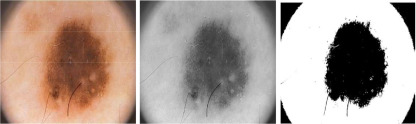
\includegraphics[width=0.38\linewidth]{images/OtsuSegmentation.jpg}
  \caption[Otsu segmentation of a dermatoscopic image]{Example of Otsu
    segmentation of a dermatoscopic image, obtained from the \(PH^2\) dataset.
    Reproduced from \cite{mendonca_ph_2013}.}
  \label{fig:otsu-dermatoscopic}
\end{figure}

To interpret an image, the most popular approach is a \textbf{convolutional neural
network (CNN)}, which learns features from labelled examples by applying small
filters learned during training \cite{lecun_gradient_1998}. Stacked layers build up
from simple edges to complex patterns, so features need not be designed by hand,
although a large dataset is needed. Each stage, from cleaning an image to finding its
structure to deciding what it shows, trades removing unwanted variation against
preserving detail, and these trade-offs matter more when images support medical
decisions.

% =====================================================================
\section{Medical Image Processing}
\label{sec:medical-imaging}

Medical images follow the same image processing as other types, but must preserve as
much anatomical detail as possible. Noise is the main threat:
\textcite{prasad_systematic_2023} state that it can degrade diagnostic quality by
blurring borders, reducing contrast and obscuring small but important details. A
common model is \textbf{Gaussian noise (GN)}, added independently to each pixel,
\begin{equation}
  I(x,y) = J(x,y) + N(x,y),
  \label{eq:gaussian-noise}
\end{equation}
where $I$ is the noisy image, $J$ is the original and $N$ is drawn from a normal
distribution with mean 0 and variance $\sigma^2$, so a larger $\sigma^2$ means
stronger noise.

The general methods of Section~\ref{sec:image-processing} were adapted for medical
use, but each involves a trade-off. Adaptive \textbf{HE} was developed for
medical image display \cite{pizer_adaptive_1987}, yet even its contrast-limited form
needs the clip limit tuned, and averaging filters suppress noise whilst blurring the
edges that carry diagnostic information. Whether an enhancement helps therefore
depends on the task: in medical imaging, quality is best defined by how well an
observer can perform a specific task, not by how the image looks
\cite{barrett_foundations_2004}. A sharper image does not necessarily lead to better
decisions, and enhancement that suits a human viewer may not help a classifier.

Because hand-designed methods depend on assumptions about the image, learned methods
have largely replaced them; a survey of over 300 studies found \textbf{CNN}s used
across medical imaging, including cardiac applications \cite{litjens_survey_2017}.
They bring their own problems. Labelled data is expensive and abnormal cases are rare,
and performance may not carry over to new data: \textcite{zech_variable_2018} found
that networks for detecting pneumonia in chest radiographs performed differently
across three hospital systems. Models may also rely on shortcuts that correlate with
the label instead of the features that matter \cite{geirhos_shortcut_2020}, and
because predictions may influence patient decisions, systems must explain their
output, for example with Grad-CAM \cite{selvaraju_gradcam_2017}, and report calibrated
confidence \cite{guo_calibration_2017}. These points apply directly to this project:
preprocessing will be judged by its effect on classification and not by appearance,
and the gap between rendered training images and real test images is a form of the
generalisation problem, with the added risk of rendering-specific shortcuts.

% =====================================================================
\section{ECG Fundamentals}
\label{sec:ecg-fundamentals}

The \textbf{ECG} is an electrical tracing of the heart, recorded non-invasively
from the surface of the body \cite{sattar_electrocardiogram_2023}. It shows how the
impulse that triggers each heartbeat spreads through the heart, so it is well suited
to detecting problems of rhythm and conduction. Each heartbeat produces a repeating
sequence of deflections (Figure~\ref{fig:ecg-beat}): the P wave reflects activation of
the atria, the QRS complex activation of the ventricles, and the T wave their
recovery. The intervals between these features carry diagnostic information: the PR
interval reflects the delay as the impulse passes from the atria to the ventricles, the
QRS duration how quickly the ventricles are activated, and the QT interval spans
ventricular activation and recovery. Abnormalities are defined by changes to these
features, so a model working from an image must find them and judge their shape and
spacing.

\begin{figure}[ht]
  \centering
  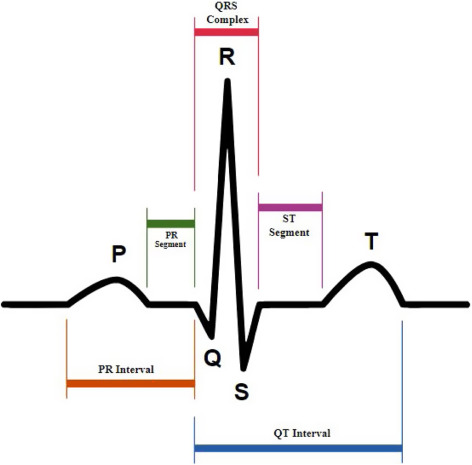
\includegraphics[width=0.35\linewidth]{images/LabelledHeartbeat.jpg}
  \caption[A single PQRST wave]{A single heartbeat, showing the P wave, QRS complex,
    T wave and main intervals. Generated by the author from
    \cite{Mazomenos_ECG_2012}.}
  \label{fig:ecg-beat}
\end{figure}

A standard resting \textbf{ECG} records twelve leads, six limb leads and six chest
leads \cite{sattar_electrocardiogram_2023}. Each lead views the same heartbeat from a
different direction, so a problem in one region of the heart often appears in only some
leads. A page cannot fit twelve full-length traces, so the printout cuts each into a
short piece and arranges them on a $3\times4$ grid \cite{ashley_conquering_2004}
(Figure~\ref{fig:ecg-grid}); a single image therefore contains twelve traces, and a
classifier must learn which leads matter for which condition. On the grid, the distance
$x$ along the paper and the deflection $y$ convert to time and voltage by $t = x/v$ and
$V = y/g$, where $v$ is the paper speed and $g$ the gain (25\,mm/s and 10\,mm/mV as
standard \cite{sattar_electrocardiogram_2023}). Clinicians read rate and intervals by
counting squares; for example, the heart rate follows from the RR interval,
\[
  \mathrm{HR} = \frac{60}{\mathrm{RR}} = \frac{300}{N},
\]
where RR is the time in seconds between successive R peaks and $N$ is the number of
large squares between them. Timing and amplitude can thus only be read from an image if
the grid calibration is known, so skewing, cropping, resizing or photographing the page
all distort it.

\begin{figure}[ht]
  \centering
  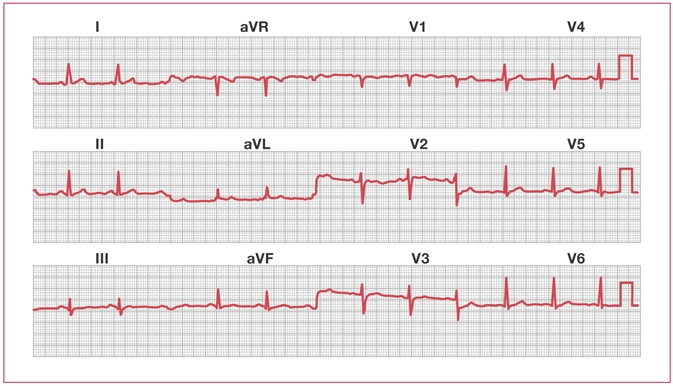
\includegraphics[width=0.4\linewidth]{images/ECGGrid.jpg}
  \caption[An ECG paper trace]{A single trace, showing a $3\times4$ grid of leads
    \cite{ashley_conquering_2004}.}
  \label{fig:ecg-grid}
\end{figure}

Clinically important abnormalities can be grouped by what they affect. Abnormal heart
rates and rhythms are known as arrhythmias \cite{nhs_heart_2018}; they include atrial
fibrillation, where beats are irregularly spaced and clear P waves are absent
\cite{van_gelder_2024_2024}, and atrial flutter, which shows a regular saw-tooth
pattern in the inferior leads \cite{cosio_atrial_2017}. Conduction disturbances such as
\textbf{bundle branch blocks (BBB)} usually widen the QRS complex \cite{scherbak_left_2024},
\textbf{myocardial infarction (MI)} and other ischaemic changes often alter the ST segment and T wave
in the leads facing the affected region, and hypertrophy of the heart's chambers is
associated with changes in amplitude \cite{channer_myocardial_2002}. Some of these
signs depend on the shape of the trace, whereas others depend on timing and regularity,
which in an image depends on the grid scale.

Public datasets encode these findings as labels. PTB-XL contains 21,837 ten-second
twelve-lead \textbf{ECG}s from about 19,000 patients, annotated by cardiologists, with diagnostic
labels grouped into five superclasses (normal, \textbf{MI}, ST/T change,
conduction disturbance and hypertrophy) plus form and rhythm statements, and a single
record can carry several labels \cite{wagner_ptbxl_2020}. It provides signals, not
images; a dataset from UMT provides real ECG images instead \cite{khan_ecg_2021}. These
fundamentals define the classes this project will detect and the two kinds of
information the classifier must use: the shape of each beat, and the timing between
beats.

\section{ECG Imaging and Digitisation}
\label{sec:ecg-imaging}

Although ECGs are recorded electronically, they are frequently printed, scanned or
photographed, and such images cannot be used directly by software that expects
time-series data \cite{shivashankara_ecg-image-kit_2024}. They also vary widely: the
ECG-Image-Database, for example, contains printed ECGs that were scanned or photographed
under different lighting conditions and camera angles, some deliberately soaked,
stained or left to grow mould, giving shadows, perspective shifts, blur, creases and
stains \cite{reyna_ecg-image-database_2024}. This is the illumination and reflectance
effect of Section~\ref{sec:image-processing}. Image resolution also limits how precisely
the trace can be read, so it directly limits the timing measurements, such as intervals
and rate, that some classes depend on.

Two approaches address the problem. Digitisation reconstructs the time-series signal
from the image so that established signal-based methods can be applied. This gives
measurable intervals, but needs several steps (locating the grid, separating the leads
and tracing each waveform), and an error at any step carries through to the
reconstructed signal. The George B.\ Moody PhysioNet Challenge 2024, for example,
evaluated digitisation by the \textbf{ signal-to-noise ratio (SNR)} of the recovered
signal \cite{physionet_challenge_2024}. The alternative is to classify the image
directly (Section~\ref{sec:ml-ecg}), which avoids reconstruction, but the model must then
learn timing from pixels, so its results depend on how the images were produced, which is
the generalisation problem of Section~\ref{sec:medical-imaging}. ECG-Image-Kit generates
synthetic ECG images from real signals, with added artefacts
\cite{shivashankara_ecg-image-kit_2024}, and the ECG-Image-Database provides 35,595
images of 1,977 recordings from PTB-XL and Emory Healthcare that were printed, degraded,
and then scanned or photographed \cite{reyna_ecg-image-database_2024}. This project
analyses ECG images directly and avoids a full digitisation step: it trains on images
rendered from PTB-XL and tests on real-world images, so that the effect of real imaging
conditions can be measured.

\section{Pre-processing and Noise Removal}
\label{sec:preprocessing}

Preprocessing corrects problems introduced during printing and capture, using the
methods of Section~\ref{sec:image-processing} matched to problems that occur in \textbf{ECG}
images, and each carries a risk. Uneven lighting and shadows can be reduced with \textbf{CLAHE}
\cite{pizer_adaptive_1987,zuiderveld_contrast_1994} or \textbf{HF}
\cite{stockham_image_1972}, at the cost of amplifying noise. Noise and specks
(Equation~\ref{eq:gaussian-noise}) can be reduced with median filtering, bilateral
filtering \cite{tomasi_bilateral_1998} or non-local means \cite{buades_non-local_2005},
although smoothing can flatten thin peaks. The printed grid can be removed by colour
segmentation or notch filtering \cite{gonzalez_digital_2018}, which struggles with faded
or monochrome prints, and rotation can be corrected by line detection, which cannot fully
undo the perspective distortion of a photograph.

The grid needs particular care because it is both noise and information: it crosses the
trace and can confuse a classifier, but it is also the only record of the time and
voltage scale (Section~\ref{sec:ecg-fundamentals}), so removing it without recording the
scale first would discard what the measurements depend on. The trace is also thin, so
smoothing or enhancement can remove P waves and sharp QRS peaks that are only a few
pixels wide. It is not certain that preprocessing helps a \textbf{CNN} at all, since a
network trained on varied, degraded images may learn to cope with them. Following the
task-based view of Section~\ref{sec:medical-imaging}, preprocessing is therefore a design
choice, judged by its effect on classification performance and not by how the image
looks.

% =====================================================================
\section{Feature Extraction}
\label{sec:features}

Before deep learning, automated \textbf{ECG} analysis relied on hand-designed features: once the
beats were located, quantities such as interval lengths and wave amplitudes were
measured and passed to a classical classifier, as in the heartbeat classification of
\textcite{de_chazal_automatic_2004}, which combined morphology and interval features.
Such features have a clear clinical meaning, which makes the model easier to explain, and
timing features are especially useful for rhythm: the regularity of the RR intervals, for
example, separates a regular rhythm from an irregular one such as atrial fibrillation. The
alternative is learned features: a \textbf{CNN} builds its features directly from pixels
\cite{lecun_deep_2015}, so no one has to decide in advance what to measure.
Hand-designed features are interpretable but depend on every earlier step succeeding,
since a missed beat or a broken trace corrupts every feature that follows; learned
features avoid this dependency but are harder to explain and need a large labelled
dataset.

This project applies both. A \textbf{CNN} learns shape-based features from the image,
which suits the set A classes. Classes defined by timing, such as heart rate and atrial
fibrillation, depend on the spacing between beats, which a model can only judge correctly
if the scale is consistent across images; measured timing features from the
waveform-detection step (Section~\ref{sec:waveform}) address this.

% =====================================================================
\section{Waveform Detection}
\label{sec:waveform}

Waveform detection finds the parts of the \textbf{ECG} that features are measured from. In digital
signals this usually means locating the QRS complex: the Pan--Tompkins algorithm does so in
real time by band-pass filtering and differentiating the signal, squaring it, smoothing it
with a moving window, and applying adaptive thresholds \cite{pan_real-time_1985}. For an
image, the first task is finding the trace itself. Published pipelines binarise the image,
remove the grid and text, repair gaps in the trace and locate each lead, using a Hough
transform to find the grid lines or lead baselines
\cite{wu_automated_2022}. Each column of the isolated trace is then
reduced to one value, for example the median vertical position of the trace pixels
\cite{wu_automated_2022}, and converted to time and voltage using the grid scale, after
which peaks can be detected as in the signal case.

Explicit detection gives measurable intervals and a rate that a clinician can check, and
it can be accurate: \textcite{randazzo_development_2022} reported an average correlation of
0.94 with reference signals on images from 16 subjects, and \textcite{wu_automated_2022}
about 99\% on standard layouts once images with overlapping leads were excluded. It is also
fragile: the correlation of \textcite{wu_automated_2022} fell to about 96\% on printed and
rescanned \textbf{ECGs}, whilst a different pipeline scored a
signal-to-noise ratio of $-2.44$\,dB on 100 rendered PTB-XL images, a poor reconstruction
by that measure. A missed or false peak changes the RR intervals and every timing feature
that follows, so errors here carry through to the prediction. This project therefore
applies waveform detection to locate the trace and the beats and supply timing features
alongside the learned image features, evaluating the detection step on real-world images
and not only on rendered ones.

\section{AI/ML Algorithms for ECG Analysis}
\label{sec:ml-ecg}

Deep learning has largely replaced feature-based methods for \textbf{ECG}classification
(Table~\ref{tab:ecg-studies}). On signals, networks reached cardiologist-level performance
on single-lead rhythm classification \cite{hannun_cardiologist_2019}, outperformed
cardiology residents on 12-lead abnormalities \cite{ribeiro_automatic_2020}, and a PTB-XL
benchmark found convolutional architectures, especially ResNet- and Inception-based ones,
performed best \cite{strodthoff_deep_2021}. Image-based work is newer.
\textcite{sangha_automated_2022} trained a \textbf{CNN} on images generated from signals
and tested it on held-out, external and printed ECGs, \textcite{gliner_domain_2023} used
domain adaptation to transfer a model to phone-captured images, and
\textcite{wang_pipeline_2025} fine-tuned a ConvNeXt backbone first on synthetic and
external images. Because labelled \textbf{ECG} images are limited, such work relies on transfer
learning, in which networks such as ResNet \cite{he_deep_2016}, pretrained on natural
images, learn general features that transfer to new tasks
\cite{yosinski_transfer_2014}.

\begin{table}[ht]
  \centering
  \footnotesize
  \caption{Key studies in deep learning for ECG classification.}
  \label{tab:ecg-studies}
  \begin{tabular}{@{}p{0.13\linewidth} p{0.27\linewidth} p{0.25\linewidth} p{0.25\linewidth}@{}}
    \toprule
    \textbf{Study} & \textbf{Input and data} & \textbf{Reported result} &
      \textbf{Limitation for this project} \\
    \midrule
    \textcite{hannun_cardiologist_2019} &
      Single-lead signals; 91,232 ECGs, 53,549 patients &
      12 rhythm classes; F1 0.837 vs.\ 0.780 for cardiologists &
      Single lead; signals, not images \\
    \textcite{ribeiro_automatic_2020} &
      12-lead signals; over two million exams &
      Six abnormalities; F1 above 80\%, specificity above 99\% &
      Signals, not images \\
    \textcite{strodthoff_deep_2021} &
      12-lead signals, PTB-XL &
      Convolutional models performed best &
      Signals; hidden weakness in subclasses \\
    \textcite{sangha_automated_2022} &
      Images generated from signals; printed ECGs to test &
      Strong performance on held-out, external and printed ECGs [TODO: AUROC] &
      Training images generated from signals [TODO: check] \\
    \textcite{gliner_domain_2023} &
      79,226 scanned labelled ECGs plus unlabelled phone-captured frames &
      Average ROC-AUC 0.91 on phone-captured images &
      Phone images made by filming printed pages; six unseen formats tested \\
    \textcite{wang_pipeline_2025} &
      Synthetic PTB-XL images plus external scanned sets &
      AUROC about 0.97 on the hidden test set &
      Synthetic test data; possible leakage from PTB-XL \\
    \bottomrule
  \end{tabular}
\end{table}

These results do not transfer directly to images. \textcite{hannun_cardiologist_2019} used
a single lead, with test labels from a consensus committee of cardiologists, and both they
and \textcite{ribeiro_automatic_2020} worked on signals, which arrive with a known sampling
rate and amplitude scale; an image carries its scale only through the printed grid, so
timing must be recovered from pixels (Section~\ref{sec:ecg-imaging}). Label quality is a
further limit. PTB-XL's labels come from at most two cardiologists
\cite{wagner_ptbxl_2020}, and agreement between cardiologists can be only poor to moderate
\cite{dhutia_interrater_2017}, so a high AUROC partly measures agreement with imperfect
labels. Studies also use different datasets, label sets and metrics (F1, specificity,
AUROC), so their headline numbers cannot be ranked directly.

Evaluation therefore needs particular care. ECG datasets are imbalanced, so accuracy can
be high even when rare but important conditions are missed; measures such as sensitivity,
specificity and the Matthews correlation coefficient give a more truthful picture
\cite{chicco_advantages_2020}, and data should be split by patient, for which PTB-XL
provides suggested folds \cite{wagner_ptbxl_2020}. A model used for decision support must
also show how far its outputs can be trusted. Modern neural networks are often
overconfident, but temperature scaling can calibrate their scores
\cite{guo_calibration_2017}. For multi-label classification each class has its own sigmoid
output, so each class score $z_k$ is divided by a temperature $T$ fitted on a held-out
validation set,
\begin{equation}
  \hat{p}_k = \sigma\!\left(\frac{z_k}{T}\right),
  \label{eq:temperature-multilabel}
\end{equation}
by minimising the binary cross-entropy of the scaled outputs. Because dividing by $T$ does
not change the ranking of scores, AUC is unaffected and only the reliability of the
probabilities changes, which is measured with the expected calibration error for each
class. Guo et al.\ described the method for single-label classification, so applying
Equation~\eqref{eq:temperature-multilabel} to independent sigmoid outputs is an
adaptation. Grad-CAM heatmaps show which image regions influenced a prediction
\cite{selvaraju_gradcam_2017}, but not why a clinician would reach the same conclusion, so
they need checking against known cases.

\section{Existing Systems and Limitations}
\label{sec:existing-systems}

Automated interpretation has been part of clinical ECG machines for decades: millions of
ECGs are recorded each year, and most are analysed by computer with an immediate report
\cite{schlapfer_computer-interpreted_2017}. However, limitations in their diagnostic
accuracy were recognised early and persist, and the authors state that over-reading and
confirmation by an experienced ECG reader are essential, because inexperienced physicians
may accept an automated reading without question
\cite{schlapfer_computer-interpreted_2017}. These systems also work on the digital signal
at the point of recording, so they cannot analyse an ECG that exists only as a printout or
image.

Deep learning systems have achieved strong results (Section~\ref{sec:ml-ecg}), but four
gaps remain that are relevant to this project. First, image-based classification has
mostly been tested on synthetic or limited real images. \textcite{gliner_domain_2023}
adapted a model to phone-captured ECGs, but their images were produced by filming printed
pages and only six unseen formats were tested, and a challenge-winning pipeline was
evaluated on synthetic images rendered from PTB-XL, which its authors note may inflate
results through data leakage \cite{wang_pipeline_2025}. Second, calibration has been
studied for signal-based atrial fibrillation detection, where uncertainty estimates
improved the expected calibration error \cite{chen_quantifying_2022}, but the image-based
studies above report discrimination measures such as AUROC. Third, explanations are seldom assessed: a review of explainable AI in cardiology found that 43\% of the studies examined did not evaluate their explanations at
all, and only 11\% involved clinicians \cite{salih_review_2024}. Fourth, how results are
presented matters and depends on the user. In interviews with 23 clinicians, accuracy
mattered more than explanation, and visualisations of what the algorithm analysed were
preferred \cite{hughes-noehrer_contrasting_2024}, while a simulated-AI experiment with 44
cardiologists found that explanations raised the trust of novices more than experts and
could mislead \cite{cabitza_painting_2023}. Datasets also reflect limited populations and
recording conditions: PTB-XL, for instance, was collected between 1989 and 1996 using
devices from a single manufacturer \cite{wagner_ptbxl_2020}, so models may not generalise
to other settings, an ethical concern discussed in the Professional, Legal, Ethical and
Social Issues section.

These gaps define the aims of this project. A preprocessing and detection pipeline tested
on real-world images addresses the first gap; a calibrated multi-label classifier
evaluated with imbalance-aware metrics addresses the second; and an application that
presents explained results to different users addresses the third and fourth.

    

\chapter{Methodology}
\label{ch:method}

\section{Research Question}

This project addresses one question: \textbf{Can a CNN, trained on rendered ECG images, detect cardiac abnormalities and rhythm disorders in real world images, and how can information and confidence be made reliable and understandable to users?}
It is broken into the objectives O1--O6 of Chapter~\ref{ch:intro}, and each method
below is linked to the objective it serves.

\section{Users and Requirements}

The main users are university students learning ECG interpretation, who need to
understand why a trace was flagged. A clinician view, which would show a short list of
flags with measured values and no teaching text, is a secondary target. The
requirements were drawn from the literature on how clinicians and users respond to
explained AI output \cite{hughes-noehrer_contrasting_2024,cabitza_painting_2023} and
from the gaps identified in Chapter~\ref{ch:lit}, and are prioritised with MoSCoW
analysis (Appendix~\ref{app:moscow}). The must-have requirements are:
upload of an ECG image; display of flagged conditions with a calibrated confidence for
each; a Grad-CAM heatmap over the original image; and a clear statement that the output
supports review and is not a diagnosis. [TODO: confirm and trim to your final must-have list.]







	\chapter{Feasibility}
\section{Coding Environment}
\section{Design}
\section{Prototypes}
\section{Datasets}
\section{Hardware}
\section{Focus Groups}

	\appendix
	

\chapter{Appendix A}

\renewcommand{\thefigure}{A.\arabic{figure}}

\section*{Scripts}


Supplementary material...



\section*{GitHub Repository}

Project planning is core aspect of any dissertation (especially for the initial groundwork).  Key tool is Git/Github



	\backmatter
	\printbibliography[heading=bibintoc,title={References}]

    \printindex

    \end{document}
	







